\section{Introduction}

\label{sec:Intro}

% Graph-- Uncertain Graph--Examples 
In emerging applications, such as business to business (B2B) and social networks,  graphs are used to capture the complex relationships inherent. Sometimes, the existence of the relationship between two entities is uncertain. For instance, in social networks, nodes represents individual users, while edges represent friendship or trust link among them.  Usually, the link is derived by inference and prediction models built on interaction details~\cite{Lin_B2B,Adar_Managing_2007,Kempe_Maximizing_2003}, and edge probability denotes the accuracy of a link prediction, or the trust of one person on another. 
In these applications, the data can be modeled and shared as uncertain graphs whose edges carries a probability of existence. The probability represents the confidence that the relationship holds in reality. 

\begin{figure}[!htb]
  \vspace{-7pt}
    \subfigure[Social Trust Network]{\label{fig:socialNetwork}
      \begin{minipage}[l]{0.46\columnwidth}
        \centering
        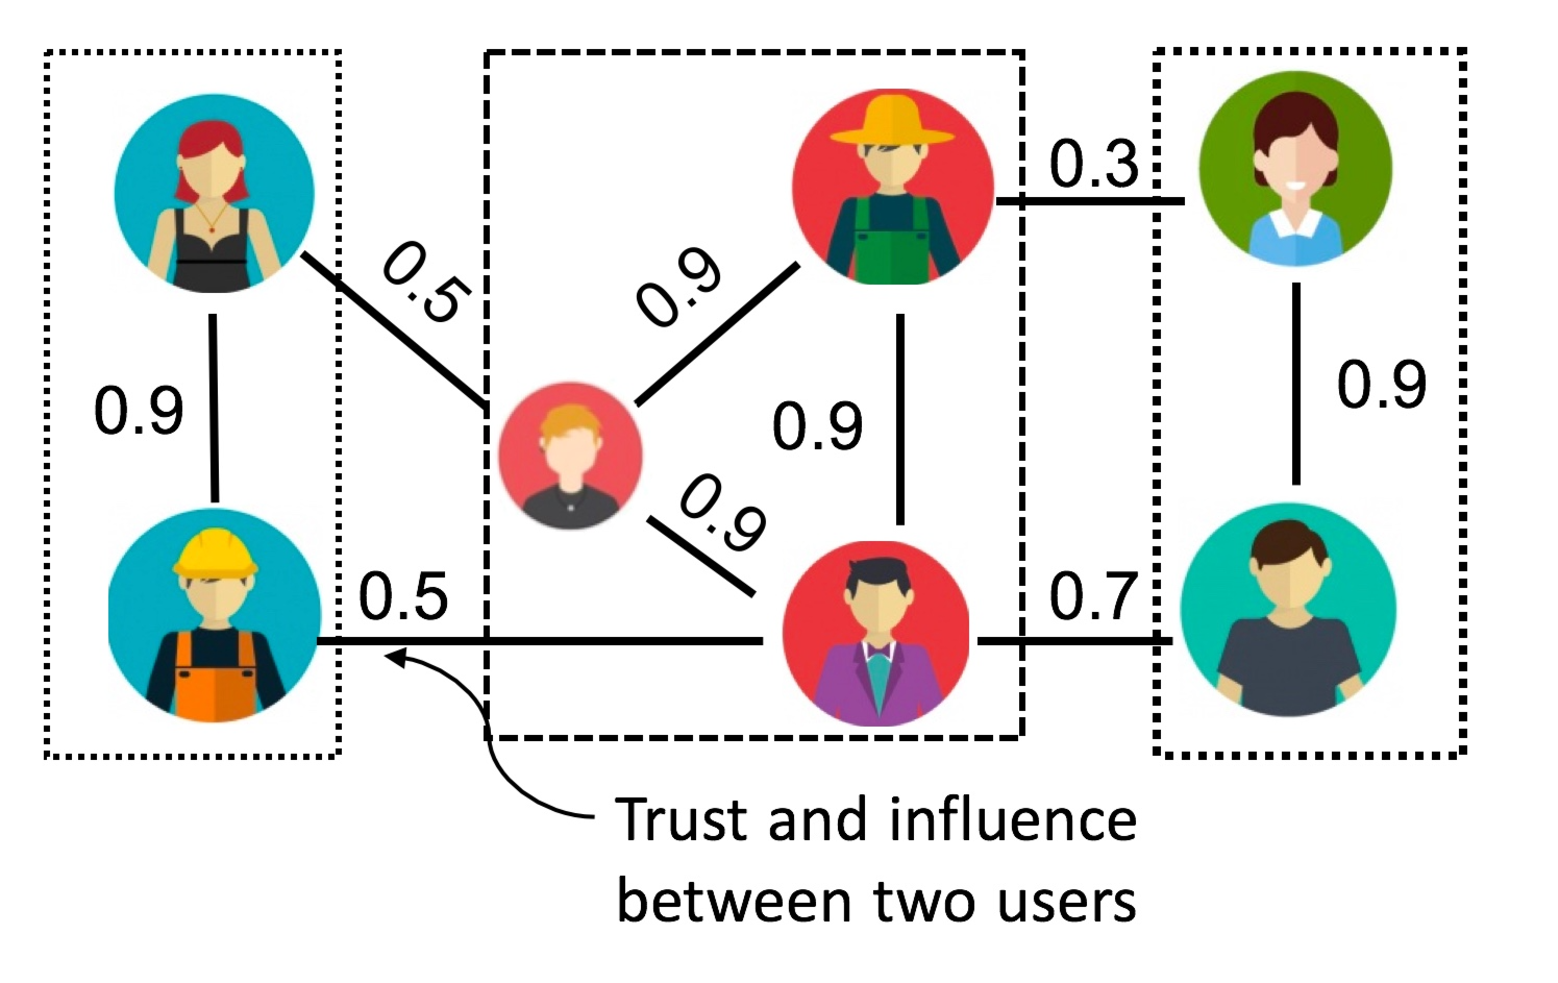
\includegraphics[height=2.7cm]{ill/SocialNetwork.pdf}
      \end{minipage}
      }
    \subfigure[B2B Network]{\label{fig:b2bNetwork}
      \begin{minipage}[l]{0.46\columnwidth}
        \centering
        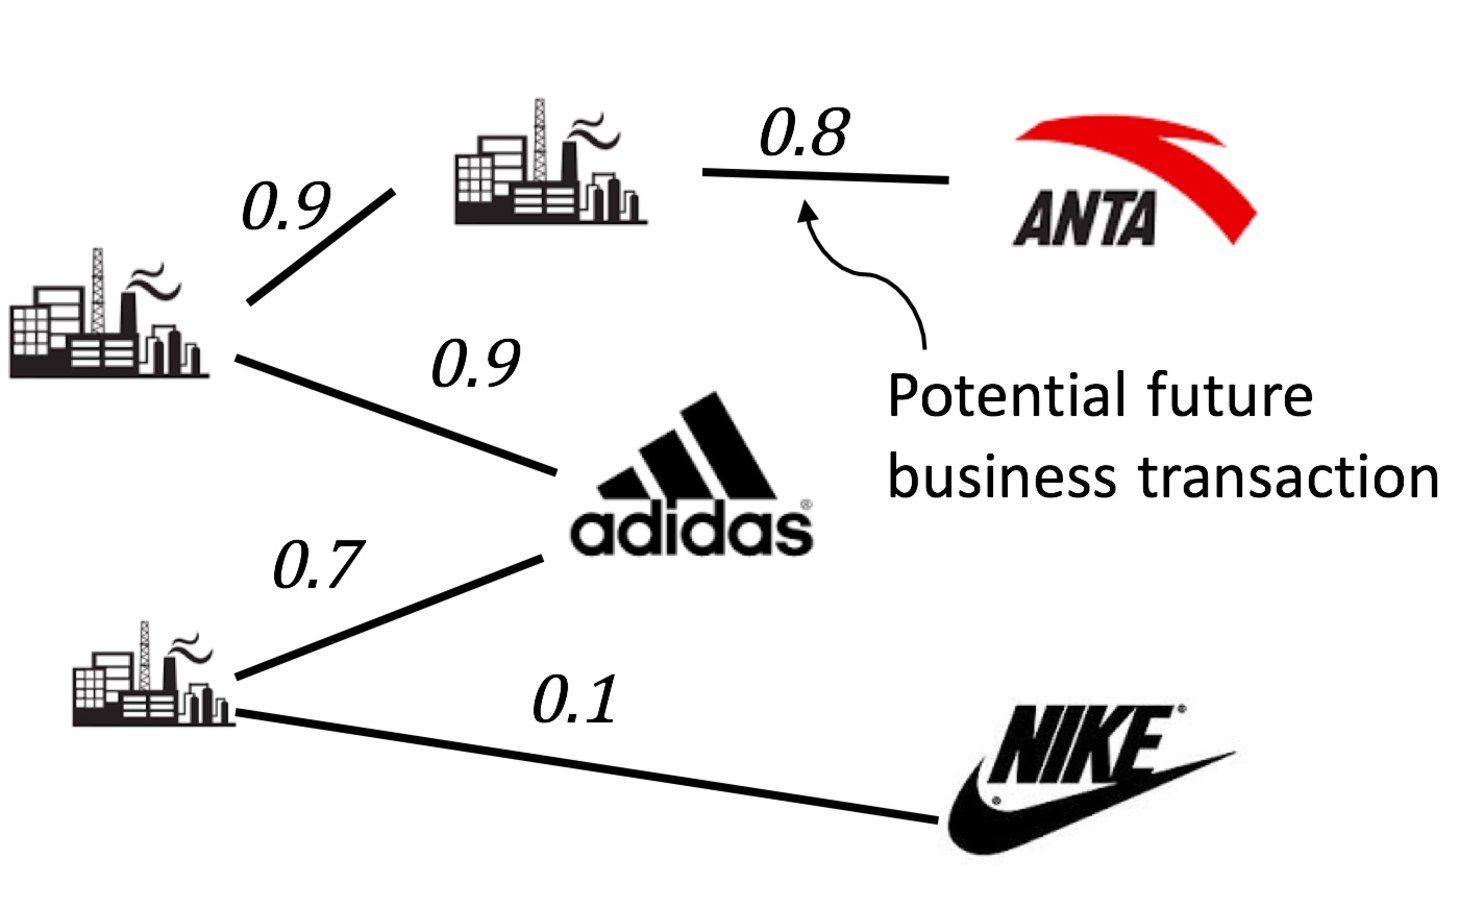
\includegraphics[height=2.7cm]{ill/B2BNetwork.pdf}
      \end{minipage}
      }
    \vspace{-7pt}
    \caption{Real-world uncertain graphs with privacy concerns.}
    \label{fig:motivation}
    \vspace{-7pt}
\end{figure} 

% Sharing--Privacy--Examples 
These uncertain graphs are invaluable for scientific research and commercial applications~\cite{Kempe_Maximizing_2003,Cho_Friendship_2011}. However, sharing these uncertain graphs would violate the privacy of users or entities profiled inside. For example, in social trust network, the trust relationships among users---which  greatly impact users' behaviors, are usually probabilistic.  They are useful in social interaction study, micro targeting. While, users are unwilling to share such confidential information with potential adversaries like Cambridge Analytica. In B2B networks, business operators also hesitate to share transaction patterns for the purpose of protecting their confidential business models. It is arising the question about sharing uncertain graphs without compromising privacy. 

% State-of-Art 
A number of privacy preserving graph sharing schemes have been studied in the deterministic scenario~\cite{Liu_Towards_2008,Ying_Randomizing_2008,Wang2011,Liu_Privacy_2009,Nguyen_Anonymizing_2015,Sala_Sharing_2011,Xiao_Differentially_2014,lee2011}, though many problems about sharing uncertain graphs still remain unexplored.

%weight casting fails 
An obvious approach is to convert uncertain graph sharing problem into the deterministic case by casting edge probabilities as edge weights. However, by disregarding the possible world semantics of the uncertain graph, such an approach fails to reflect uncertain graph properties such as connectivity, dense subgraphs correctly~\cite{Zhao_Detecting_2014,Hua_Probabilistic_2010}. {\small Note that connectivity of deterministic subgraphs is generally measured by the concept of cut, which is defined as the sum of weights of intra edges. Generally, the bigger the cut, the harder to separate two subgraphs. In Figure~\ref{fig:socialNetwork}, the equal cut $C(SG_{1},SG_{2})=C(SG_{3},SG_{2})=1$ implies the identical connectivity of $SG_{1}$ and $SG_{3}$ w.r.t $SG_{2}$. However, with the possible world semantics, we know the probability to separate $SG_{1}$ and $SG_{2}$ is $(1-0.5)^{2}=0.25$, and that to separate $SG_{2}$ and $SG_{3}$ is $(1-0.3)(1-0.7)=0.21$. Hence, in fact, $SG_{2}$ is closer to $SG_{1}$ than to $SG_{3}$.} 
Hence, the weighted graph anonymization scheme could produce very poor result in the uncertain scenario even if the anonymization algorithm is good. 


% Rep-OB 
In previous work~\cite{Xiao:2018}, we ever present another option (Rep-An) which replaces the given uncertain graph with its single representative instance. It enables the use of existing graph anonymization methods in the uncertain scenario, regardless of the uncertainty.  Yet, this approach is shown to be problematic. The detachment of probabilities in the first step deteriorates the data utility. 

As ever mentioned, either the casting or detachment of edge probabilities lead to poor results. Existing graph anonymization schemes are inadequate to share uncertain graph with desirable trade-off between privacy and utility. 
In contrast, our work seeks a solution tailored towards uncertain graphs via incorporating possible world semantics. We develop {\methodName} on the basis of syntactic private notation. {\methodName} preserves as much the stochastic nature of the original uncertain graph as possible, while injecting enough structural noise to guarantee a chosen level of privacy against re-identification attacks. To achieve above goals, we carefully addressed following issues. 

$\bullet$~\textup{\emph{Stochastic Privacy Attacks.}}~~In the uncertain graph model, edge uncertainty plays an indispensable role. It is impractical to discard them in the release.  
While, the extra release of edge uncertainty makes privacy protection far more difficult as it  empowers the adversary and make the profiled entity more vulnerable. To this end, we show the potential re-identification attack and present the corresponding solution. 

$\bullet$~\textup{\emph{Stochastic Utility Loss Metric.}}~~It is very challenging to maintain the graph structure when the uncertain graph is modified to pursue anonymity. The utility loss incurred by the distortion is evaluated according to metrics. Unfortunately, existing graph utility loss metrics such as graph edit distance~\cite{Liu_Towards_2008}, spectrum discrepancy~\cite{Ying_Randomizing_2008}, community reconstruction error~\cite{Wang2011} and shortest path discrepancy~\cite{Liu_Privacy_2009} are not suitable in the uncertain scenario because of the ignorance of edge probability. In this context, the discrepancy w.r.t standard uncertain graph reliability become a good criterion. It evaluates the connectivity difference in the context of the entire graph and meanwhile utilizes the possible world model. 

$\bullet$~\textup{\emph{Intractable Search Space.}}~~It is very challenging to find a sanitized graph with the desired level of privacy by as few graph contractions as possible. In the deterministic scenario, it is NP-hard with edge addition and edge deletion operations\cite{Hartung_Theory_2015}. In the uncertain scenario, the edge modification is no longer a binary operation (addition/deletion), but can be infinite probability values. Exhaustive search is computationally intractable if the number of edges is large. Thus, we approximate the problem of interest via a randomized algorithm, which built on the basis of meta-heuristics. It excels in identifying a population of sanitized results with good quality.

The rest of the paper is organized as follows. In Section 2, we summarize related works and clarify our distinct  privacy  goal. In Section 3 we formulate the uncertain graph-anonymization problem. Sections 4 – 5 consider the anonymization problem in the context of uncertain graphs.  In Section 6 we apply our method to several real-world uncertain graphs, and demonstrate their efficiency and practical utility. 
